\documentclass[12pt]{article}
\usepackage[margin=0.75in]{geometry}
\usepackage{mathptmx}
\usepackage{graphicx}
\usepackage{amsmath}
\usepackage{amssymb}
\usepackage{setspace}
\usepackage{booktabs}
\usepackage[hidelinks]{hyperref}
\usepackage{url}
\usepackage{caption}
\usepackage[T1]{fontenc}

\singlespacing
\setlength{\parindent}{0.5in}
\setlength{\parskip}{2pt}
\captionsetup{font=small, labelfont=bf}

\begin{document}

% ---------------------------------------------------------------
%  TITLE
% ---------------------------------------------------------------
\begin{center}
{\fontsize{14}{16.8}\selectfont
  \textbf{System Identification of a Nonlinear Two-Mass Spring-Damper System:\\[2pt]
          Least Squares vs.\ Recurrent Neural Network}}
\end{center}
\vspace{2pt}

% ---------------------------------------------------------------
%  BODY
% ---------------------------------------------------------------

In this lab rotation, I worked with Prof. Caines on system identification of a nonlinear two-mass, two-spring,
two-damper mechanical system, comparing classical least-squares (LS) against Recurrent Neural Networks (RNNs), motivated by the paper in~\cite{revay2021}.
The system has two carts connected in series to a fixed wall, each coupled to a nonlinear hardening spring with piecewise-linear function $\Gamma(d)$ along with a damper (see Appendix~A for all governing equations). An external piecewise-constant force $u(t)$ drives Cart~1.
The state vector is $\mathbf{x}=[x_1,\dot{x}_1,x_2,\dot{x}_2]^{\top}$ with
$m=[\tfrac{1}{4},\tfrac{1}{3}]$\,kg, $c=[\tfrac{1}{4},\tfrac{1}{3}]$\,Ns/m,
$k=[1,\tfrac{5}{6}]$\,N/m (matching the reference paper). All code is at~\cite{code}.

For the first phase, I started with data generation and Least Squares (LS) baselines. I simulated two spring variants (Fig. \ref{springs profile}). The original system has a deadzone threshold, $\delta{=}1.0$, and a shrunk variant with $\delta{=}0.25$ (as suggested by Prof. Caines). Here, the spring enters a steeper linear region at much smaller displacements. For each variant, I generated a training trajectory (with seed~42, Fig. \ref{original non lin springs with delta 1}) and a held-out test trajectory
(seed~99) using RK4 integration ($\Delta t{=}0.01$\,s, $T{=}200$\,s, 20\,000 steps).
I used both the raw states $\mathbf{x}$ and relative coordinates
$\mathbf{z}=[x_1{-}x_2,\,\dot{x}_1{-}\dot{x}_2,\,x_2,\,\dot{x}_2]^{\top}$ to test my LS models. As a quantitative measure for model quality, I used NSE as defined in the paper: ~$\|\hat{y}{-}y\|/\|y\|$ (lower is better;
NSE~$>1$ means divergence). I also implemented the Auto Regressive Moving Average (ARMA) for the LS approach. The ARMA predictor uses $\mathbf{x}_{k+1}=D\mathbf{x}_k+E_1 u_{k+1}+E_2 u_k$
to fit by pseudoinverse on all four combinations of data (Table~1, Appendix~A).
On the original raw springs, the LS model performs better in closed-loop rollout in either coordinate system (with test NSE$\approx$0.20 for raw data, and 0.31 for transformed $z$; Figs. \ref{ls model on raw data} -- \ref{ls model on transformed z data}) but it does not have perfect scores as a linear approach cannot model the deadzone's nonlinearity perfectly. We apply the same procedure to the shrunk springs, and it yields substantially lower NSE (test~0.08 raw, 0.15 transformed; Fig. \ref{ls on shrunk} -- \ref{ls on shrunk z transformed}): with $\delta{=}0.25$ as the system spends most of its time in the linear region, making the overall linear approximation much more accurate than $\delta {=} 1.0$.

Next, I switched to the RNN. I initially built a vanilla open-loop Elman RNN ($h_k=\tanh(h_k W_{hh}+u_k W_{uh}+b_h)$,
hidden size~32, 3,000 epochs), tracked the ground truth given true inputs at each step
(Fig. \ref{open loop vanilla RNN}) but it soon diverged immediately in autonomous rollout as the errors compound through the feedback path. So I redesigned the RNN's forward function to implement a closed-loop autoregressive model. This new model receives $[\mathbf{z}_k;\,u_k]\in\mathbb{R}^5$, predicts
$\hat{\mathbf{z}}_{k+1}$, and that prediction feeds back as the next input.
Working in transformed $\mathbf{z}$-coordinates (hidden~64, batch~16, Adam
$\text{lr}{=}10^{-4}$, gradient clipping), I compared four activations:
\textbf{ReLU} (Fig. \ref{CL RNN loss}--\ref{CL RNN trajectory}), \textbf{ELU} (Fig. \ref{CL ELU RNN trajectory}), \textbf{tanh} (Fig. \ref{CL tanh RNN trajectory}), and a
physics-inspired deadzone variant (\textbf{NLT}) before the hidden update,
$z_1$ is replaced by $\text{deadzone}(z_1,1.0)$, zeroing the soft spring region to
expose the underlying stiff dynamics more directly to the network (Fig. \ref{CL NLT RNN trajectory}).

% For the next phase of the project, I implemented two experiments: 2a and 2b. Experiment 2a (Figs. \ref{2a training loss}--\ref{2a eval}) used the best closed-loop ReLU configuration
% (h=64, z-coords) but added a \texttt{ReduceLROnPlateau} scheduler (initial
% $\text{lr}{=}0.01$, factor~0.5, patience~50 epochs). Training loss reached a minimum
% of $1.47\times10^{-4}$ over 1\,000 epochs, and the LR went from~0.01
% down to $3.9\times10^{-5}$ across seven reductions.
% Despite this, the autoregressive NSE exceeded 1.7 on both the training and test sets (indicating divergence). The one-step teacher-forcing with a decaying LR over-optimizes for small loss but produces a closed-loop system that is not autonomously stable. Experiment 2b (Figs. \ref{2b loss}--\ref{2b eval}) addressed this with a physics-informed residual/error
% architecture where the 9-dim input $[\mathbf{z}_k;\,u_k;\,\hat{\mathbf{z}}_{k+1}^{\text{LS}}]$
% adds to the state with the LS model's forward prediction. Now the RNN only needs to learn
% the nonlinear residual: $\Delta\hat{\mathbf{z}}_{k+1}=\hat{\mathbf{z}}_{k+1}-\hat{\mathbf{z}}_{k+1}^{\text{LS}}$.
% With the same LR scheduler the model converged stably, reaching test NSE
% $z_1{=}0.40$, $z_3{=}0.20$. This is the best RNN result, with $z_3$ matching the LS
% baseline on the absolute coordinate.

In the next phase, I experimented with two approaches: 2a and 2b. For 2a (Figs. \ref{2a training loss}--\ref{2a eval}) I used the best closed-loop ReLU configuration (h=64, z-coords) with a \texttt{ReduceLROnPlateau} scheduler (initial $\text{lr}{=}0.01$, factor~0.5, patience~50). Training loss reached $1.47\times10^{-4}$ over 1,000 epochs, with the LR dropping to $3.9\times10^{-5}$. Despite this, the autoregressive NSE exceeded 1.7 on both sets. This shows that one-step teacher-forcing with a decaying LR over-optimizes for small loss but lacks stability. Approach 2b (Figs. \ref{2b loss}--\ref{2b eval}) solved this using a physics-informed residual architecture. By feeding the 9-dim input $[\mathbf{z}_k;\,u_k;\,\hat{\mathbf{z}}_{k+1}^{\text{LS}}]$, the RNN only learns the nonlinear residual: $\Delta\hat{\mathbf{z}}_{k+1}=\hat{\mathbf{z}}_{k+1}-\hat{\mathbf{z}}_{k+1}^{\text{LS}}$. With the same scheduler, the model converged stably (test NSE: $z_1{=}0.40$, $z_3{=}0.20$), making this the best RNN result and matching the Z-coordinate LS baseline for $z_3$.

% Overall, these experiments reveal that LS is the most efficient baseline and is optimal for dynamic systems where closed-loop training is necessary but not sufficient for stability. Feeding back the
% RNN input with the LS prediction (Exp.~2b) is the most effective approach tested. My future work can include implementing convex parametrization to improve robustness of the vanilla RNN, as suggested in \cite{revay2021}, and extending the study to the full four-mass system.

Ultimately, these experiments reveal that LS is a highly efficient baseline and that feeding back the LS prediction into the RNN (Exp.~2b) is the most effective RNN method tested. My future work can explore convex parameterization to improve the robustness of the vanilla RNN, like in \cite{revay2021}, and extend the study to the full four-mass system.

% ---------------------------------------------------------------
%  REFERENCES  (on new page, like previous rotation report)
% ---------------------------------------------------------------
\newpage
\begin{thebibliography}{9}
\setlength{\itemsep}{2pt}
\setlength{\parsep}{0pt}
\bibitem{revay2021}
  M.~Revay, R.~Wang, and I.~R.~Manchester,
  ``A convex parameterization of robust recurrent neural networks,''
  \textit{IEEE Control Systems Letters}, vol.~5, no.~4, pp.~1363--1368, Oct.~2021.

\bibitem{code}
  O.~Gundra, ``RNN Honours Rotation,'' GitHub, 2026. [Online].
  Available: \url{https://github.com/BraveKing15/RNN-Honours-Rotation}
\end{thebibliography}

% ---------------------------------------------------------------
%  APPENDIX A  –  Governing Equations & LS Table
% ---------------------------------------------------------------
\newpage
\section*{Appendix A: Governing Equations and Results Summary}

\noindent\textbf{Nonlinear Spring Profile ($\delta$~=~threshold):}
\begin{equation}
  \Gamma(d;\delta) =
  \begin{cases}
    d + 0.75\delta & d \leq -\delta \\
    0.25\,d        & |d| < \delta   \\
    d - 0.75\delta & d \geq \delta
  \end{cases}
  \quad\text{(original: }\delta{=}1.0,\text{ shrunk: }\delta{=}0.25\text{)}
\end{equation}

\noindent\textbf{Equations of Motion (RK4, $\Delta t=0.01$\,s):}
\begin{align}
  m_1\ddot{x}_1 &= u - k_1\gamma(x_1) - c_1\dot{x}_1 + k_2\gamma(x_2-x_1) + c_2(\dot{x}_2-\dot{x}_1) \\
  m_2\ddot{x}_2 &= -k_2\gamma(x_2-x_1) - c_2(\dot{x}_2-\dot{x}_1)
\end{align}

\noindent\textbf{LS ARMA Predictor (pseudoinverse):}
\begin{equation}
  \mathbf{x}_{k+1} = D\mathbf{x}_k + E_1 u_{k+1} + E_2 u_k = \Theta\,[\mathbf{x}_k;\,u_{k+1};\,u_k], \qquad
  \Theta = X_{\text{next}}\,Z^\top(ZZ^\top)^{-1}
\end{equation}

\noindent\textbf{Closed-Loop Autoregressive RNN:}
\begin{align}
  h_{k+1} &= \sigma\bigl(h_k W_{hh} + [\mathbf{z}_k;\,u_k]\,W_{uh} + b_h\bigr), \quad
  \hat{\mathbf{z}}_{k+1} = h_{k+1}W_{hx} + b_x, \quad \mathbf{z}_{k+1}\leftarrow\hat{\mathbf{z}}_{k+1}
\end{align}

\noindent\textbf{Physics-Informed Residual (Exp.~2b, input size~9):}
\begin{equation}
  \hat{\mathbf{z}}_{k+1} =
    \underbrace{D\mathbf{z}_k+E_1 u_{k+1}+E_2 u_k}_{\hat{\mathbf{z}}_{k+1}^{\text{LS}}}
    + \text{RNN}\bigl([\mathbf{z}_k;\,u_k;\,\hat{\mathbf{z}}_{k+1}^{\text{LS}}]\bigr)
\end{equation}

\vspace{8pt}
\noindent\textbf{Table 1: Normalized Simulation Error (NSE) Summary.}
Lower is better. NSE~$>1$ indicates divergence worse than predicting zero.

\vspace{4pt}
\begin{center}
\small
\begin{tabular}{lcc}
\toprule
\textbf{Method} & \textbf{Train NSE (avg)} & \textbf{Test NSE (avg)}  \\
\midrule
\textit{Least Squares} & & \\
\quad Original $\pm1.0$ --- raw $\mathbf{x}$       & 0.1693 & 0.2001 \\
\quad Original $\pm1.0$ --- transformed $\mathbf{z}$ & 0.2553 & 0.3089 \\
\quad Shrunk $\pm0.25$ --- raw $\mathbf{x}$         & 0.0631 & 0.0795 \\
\quad Shrunk $\pm0.25$ --- transformed $\mathbf{z}$  & 0.1181 & 0.1542 \\
\midrule
\textit{RNN (closed-loop, transformed $\mathbf{z}$, $n_h{=}64$)} & & \\
\quad Exp.~2a: ReLU + LR Scheduler       & $>1.7$ & $>1.7$ \;(diverges) \\
\quad Exp.~2b: LS Residual + LR Scheduler & $\approx0.27$ & $\approx0.30$ \\
\bottomrule
\end{tabular}
\end{center}

% ---------------------------------------------------------------
%  APPENDIX B  –  Phase 1: Data & LS Figures
% ---------------------------------------------------------------
\newpage
\section*{Appendix B: Graphs and Data}

\begin{figure}[h!]
  \centering
  
\includegraphics[width=0.85\textwidth]{2 spring regions.png}
  \caption{Spring Force Profiles.
    Left: original spring ($\delta{=}1.0$) with a deadzone. Right: shrunk spring ($\delta{=}0.25$), which enters the steeper linear region 
    at much smaller displacements. The shrunk variant is more linear over typical amplitude ranges, making LS identification easier.}
    \label{springs profile}
\end{figure}

\begin{figure}[h!]
  \centering
  
\includegraphics[width=\textwidth]{Original non linear springs with delta 1.png}
  \caption{Training vs.\ Test Trajectories (Original Springs, $\delta{=}1.0$).
    Left: training data (seed~42). Right: held-out test data (seed~99).
    Both use piecewise-constant input forces (switching every 5\,s) over 200\,s.}
    \label{original non lin springs with delta 1}
\end{figure}

\begin{figure}[h!]
  \centering
  
\includegraphics[width=\textwidth]{Shrunk non linear springs.png}
  \caption{Training vs.\ Test Trajectories (Shrunk Springs, $\delta{=}0.25$).
    Similar input. The reduced deadzone causes the system to settle faster with smaller oscillations compared to the original spring variant.}
\end{figure}

\begin{figure}[h!]
  \centering
  
\includegraphics[width=\textwidth]{LS on original non linear springs raw states.png}
  \caption{LS Model: Original Springs, Raw States.
    Train (left) and test (right) autoregressive rollout.
    NSE: Cart~1 train/test $\approx0.15/0.18$, Cart~2 train/test $\approx0.18/0.22$.
    The model approximately tracks the trajectory but diverges in the soft nonlinear region.}
    \label{ls model on raw data}
\end{figure}

\begin{figure}[h!]
  \centering
  
\includegraphics[width=\textwidth]{LS on original non linear springs transformed z states.png}
  \caption{LS Model: Original Springs, Transformed $\mathbf{z}$-Coordinates.
    Train/test NSE: $z_1\approx0.32/0.40$, $z_3\approx0.18/0.22$.
    The coordinate transformation does not improve the closed-loop fit. The nonlinearity
    is intrinsic and cannot be resolved by re-parameterization alone.}
    \label{ls model on transformed z data}
\end{figure}

\begin{figure}[h!]
  \centering
  
\includegraphics[width=\textwidth]{LS on shrunk non linear springs.png}
  \caption{LS Model on Shrunk Springs ($\delta{=}0.25$), Raw States.
    Train/test NSE: Cart~1~$\approx0.05/0.07$, Cart~2~$\approx0.07/0.09$.
    Substantially better than the original springs since the system frequently stays in the linear region, making the global linear model a better fit.}
    \label{ls on shrunk}
\end{figure}

\begin{figure}[h!]
  \centering
  
\includegraphics[width=\textwidth]{LS on shrunk non linear springs with transformed.png}
  \caption{ LS Model: Shrunk Springs ($\delta{=}0.25$), Transformed $\mathbf{z}$.
    Train/test NSE: $z_1\approx0.16/0.21$, $z_3\approx0.07/0.09$. Almost no improvement over the original springs. Identical performance to the raw-state LS on the same data, confirming the transformation does not consistently help.}
    \label{ls on shrunk z transformed}
\end{figure}

% ---------------------------------------------------------------
%  APPENDIX C  –  RNN Activation Function Comparison
% ---------------------------------------------------------------
% \newpage
% \section*{Appendix C: RNN Exploration --- Open-Loop and Activation Comparisons}

\begin{figure}[h!]
  \centering
  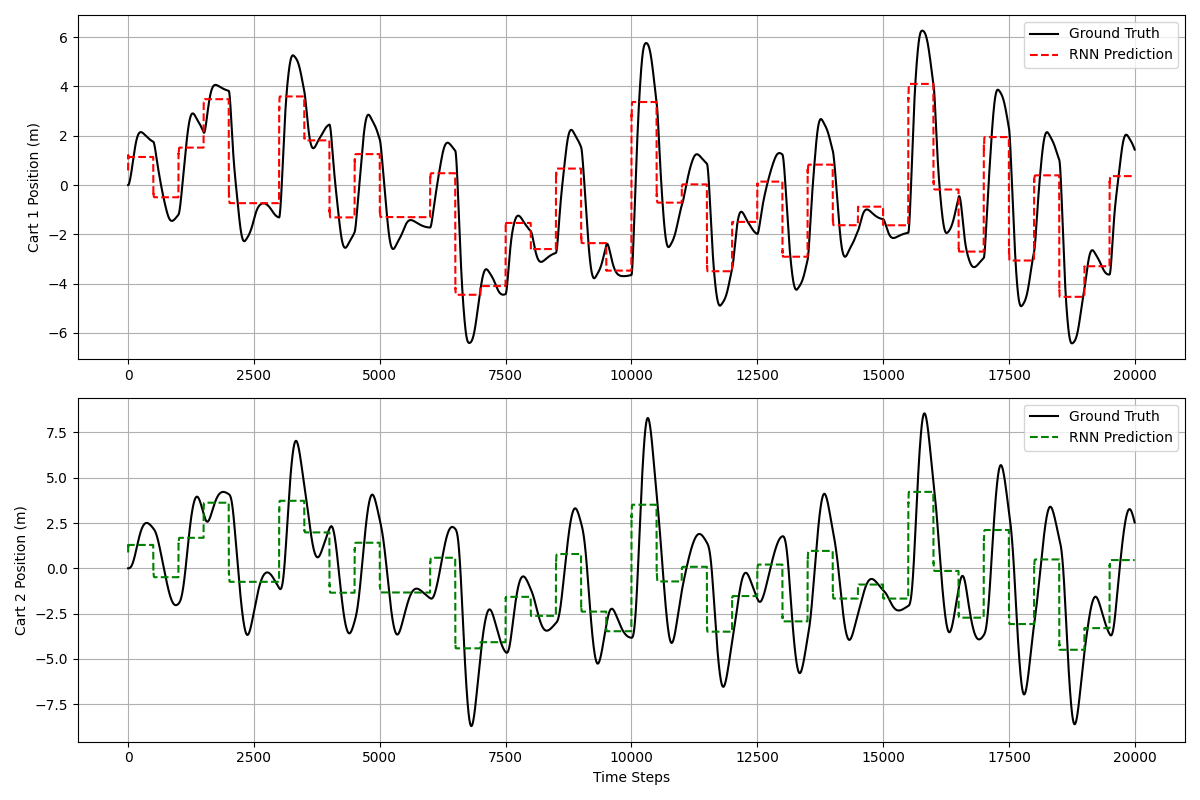
\includegraphics[width=\textwidth]{Vanilla RNN Comparison.png}
  \caption{Open-Loop Vanilla RNN (hidden~32, tanh, raw states).
    Given the true input $u(t)$ at each step the model tracks the ground truth for
    both carts. However, this model diverges immediately when rolled out autoregressively,
    as prediction errors compound through the feedback path.}
    \label{open loop vanilla RNN}
\end{figure}

\begin{figure}[h!]
  \centering
  
\includegraphics[width=0.7\textwidth]{CL RNN Loss.png}
  \caption{CL ReLU RNN Training Loss (hidden~64 (mistake in the image)), $\mathbf{z}$-coords, $n_\text{epochs}=1000$).
    Loss decreases from $\approx0.2$ to $\approx0.0015$ over 1\,000 epochs with
    Adam ($\text{lr}{=}10^{-4}$) and gradient clipping.}
    \label{CL RNN loss}
\end{figure}

\begin{figure}[h!]
  \centering
  
\includegraphics[width=\textwidth]{CL RNN Trajectory.png}
  \caption{CL ReLU RNN Evaluation (hidden~64, $\mathbf{z}$-coords).
    Train and test were both done on the same dataset, yet sthe autoregressive rollout on $z_1$ (relative position) and $z_3$ (Cart~2 absolute position) still performs poorly on the already seen data.}
    \label{CL RNN trajectory}
\end{figure}

\begin{figure}[h!]
  \centering
  
\includegraphics[width=\textwidth]{CL ELU RNN Trajectory.png}
  \caption{CL ELU RNN Evaluation (hidden~64, $\mathbf{z}$-coords).
    Same architecture and training as Fig. \ref{CL RNN trajectory} but with ELU activation. ELU's smooth
    negative saturation provides slightly different gradient flow but similar autoregressive tracking performance.}
    \label{CL ELU RNN trajectory}
\end{figure}

\begin{figure}[h!]
  \centering
  
\includegraphics[width=\textwidth]{CL tanh RNN Trajectory.png}
  \caption{CL tanh RNN Evaluation (hidden~64, $\mathbf{z}$-coords).
    tanh activation with the same closed-loop setup. The bounded output of tanh
    ($\in(-1,1)$) provides natural clipping but can suffer from vanishing gradients
    for large hidden sizes.}
    \label{CL tanh RNN trajectory}
\end{figure}

\begin{figure}[h!]
  \centering
  
\includegraphics[width=\textwidth]{CL NLT RNN Trajectory.png}
  \caption{CL Deadzone/NLT RNN Evaluation (hidden~64, $\mathbf{z}$-coords).
    The physics-inspired deadzone transform ($z_1\!\leftarrow\!\text{deadzone}(z_1,1.0)$)
    is applied to the relative position state before the hidden update, zeroing values
    in the deadzone region. This is a form of physics-informed feature engineering
    that exposes the steep linear spike in the spring structure more directly to the network.}
    \label{CL NLT RNN trajectory}
\end{figure}

% ---------------------------------------------------------------
%  APPENDIX D  –  Phase 2 Experiments
% ---------------------------------------------------------------
% \newpage
% \section*{Appendix D: Phase 2 --- LR Scheduler \& Physics-Informed Residual}

\begin{figure}[h!]
  \centering
  
\includegraphics[width=0.85\textwidth]{2a train loss.png}
  \caption{2a Training Loss \& LR Schedule (ReLU, h=64, scheduler).
    Top: training MSE loss on log scale. Bottom: \texttt{ReduceLROnPlateau} schedule. The LR halves each time the loss stagnates for 50~epochs, decreasing from~0.01 to $3.9\times10^{-5}$ across seven reductions. Minimum loss: $1.47\times10^{-4}$.}
    \label{2a training loss}
\end{figure}

\begin{figure}[h!]
  \centering
  
\includegraphics[width=\textwidth]{2a eval.png}
  \caption{2a Autoregressive Evaluation (divergence).
    Despite the low training loss, the closed-loop rollout diverges on both train (left)
    and test (right) data: NSE~$z_1{=}1.75$, $z_3{=}1.77$ (train);
    $z_1{=}1.75$, $z_3{=}1.55$ (test). This reveals that an aggressive decrease in the LR over-optimizes the teacher-forced procedure, but the learned recurrence is not autonomously stable.}
    \label{2a eval}
\end{figure}

\begin{figure}[h!]
  \centering
  
\includegraphics[width=0.85\textwidth]{2b Loss.png}
  \caption{2b Training Loss \& LR Schedule (LS Residual, h=64).
    Same \texttt{ReduceLROnPlateau} as 2a but with 9-dim input $[\mathbf{z}_k;\,u_k;\,\hat{\mathbf{z}}_{k+1}^{\text{LS}}]$. Minimum loss: $1.97\times10^{-4}$. The loss converges similarly, but the residual/error  stabilizes over the autonomous rollout.}
    \label{2b loss}
\end{figure}

\begin{figure}[h!]
  \centering
  
\includegraphics[width=\textwidth]{2b eval.png}
  \caption{2b Autoregressive Evaluation (best RNN result).
    The physics-informed residual model achieves stable closed-loop rollout:
    NSE~$z_1{=}0.35$, $z_3{=}0.18$ (train);
    $z_1{=}0.40$, $z_3{=}0.20$ (test). The absolute position $z_3$ matches
    the LS test baseline (0.20). By providing the LS prediction as an extra input
    feature, the RNN learns only the nonlinear correction, greatly improving
    autonomous stability compared to 2a.}
    \label{2b eval}
\end{figure}

\end{document}
